\chapter{Interfejs użytkownika i funkcje końcowe}
\label{ch:interfejs_uzytkownika}
\raggedbottom
Niniejszy rozdział opisuje warstwę użytkową aplikacji VT-LAN: układ
ekranów, przepływ pracy użytkownika oraz funkcje dostępne w finalnej
wersji programu. Omówiono kolejne etapy rozwoju interfejsu - od widoku
diagnostycznego po kompletny przepływ obejmujący ekran startowy, formularze
sesji i główny pokój rozmowy - a także szczegóły mechanizmu zaproszeń,
obsługi czatu i przesyłania plików.

Techniczne szczegóły implementacji poszczególnych komponentów
(biblioteka ImGui, obsługa drag-and-drop w SDL3, protokół \texttt{vtlan://},
system RPC) opisano w rozdziale~\ref{chapt:Backend}.

% ─────────────────────────────────────────────────────────────────────────────
\section{Założenia projektowe interfejsu}
\label{sec:zalozenia_ui}
% ─────────────────────────────────────────────────────────────────────────────

Celem warstwy interfejsu było przygotowanie czytelnego widoku do obsługi
rozmowy głosowej, czatu i przesyłania plików, przy zachowaniu minimalnego
narzutu zasobów i prostego modelu obsługi. Przyjęto zasadę minimalizmu
funkcjonalnego - każdy widoczny element powinien pełnić konkretną rolę
w podstawowym scenariuszu pracy, a funkcje wykraczające poza ten zakres
(wideo, transmisja ekranu, konta w chmurze) pozostawiono jako kierunki
dalszej rozbudowy.

Projekt wizualny opiera się na ciemnym motywie z fioletowymi akcentami
wyznaczającymi przyciski akcji, co ułatwia szybkie zlokalizowanie
elementów klikalnych i zmniejsza zmęczenie wzroku podczas dłuższej pracy.
Układ ekranu jest stały i przewidywalny: lewa część odpowiada za
komunikację głosową, prawa za czat i pliki.

% ─────────────────────────────────────────────────────────────────────────────
\section{Inspiracje projektowe}
\label{sec:inspiracje_ui}
% ─────────────────────────────────────────────────────────────────────────────

Podczas projektowania przeanalizowano rozwiązania zastosowane w popularnych
komunikatorach omówionych w sekcji~\ref{sec:przeglad_rynku}. Poniższe
rysunki przedstawiają schematyczne odwzorowania ekranów referencyjnych,
których celem jest zilustrowanie układu funkcji - nie kopiowanie cudzych
interfejsów.

\begin{figure}[H]
	\centering
	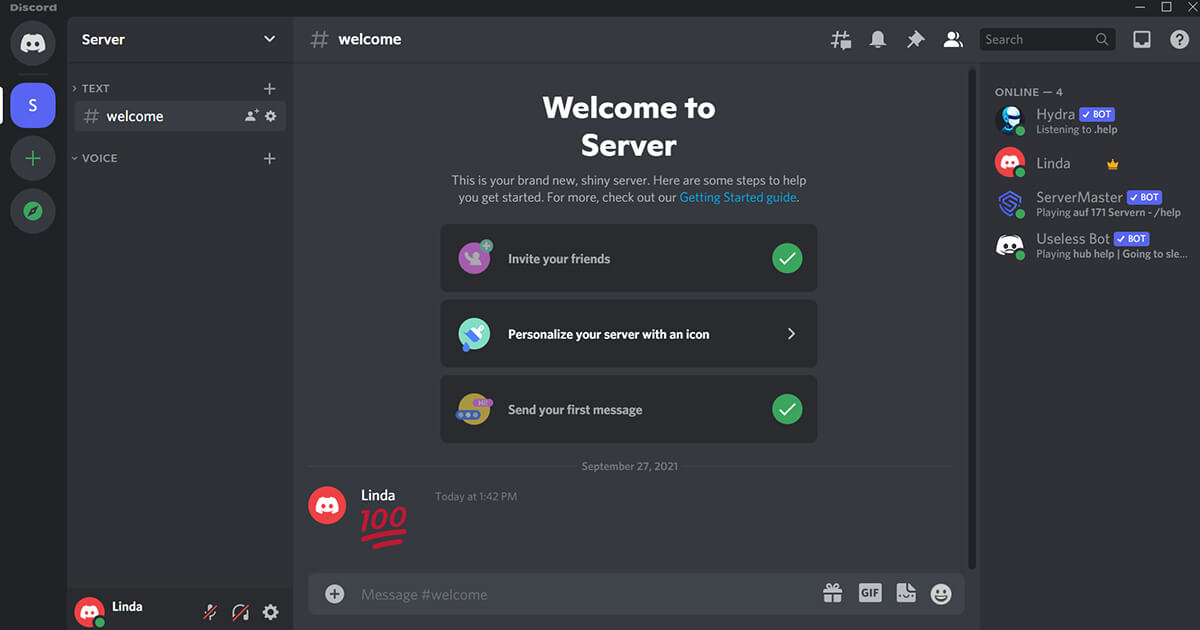
\includegraphics[width=0.95\textwidth,keepaspectratio]{figures/chapter3/ch3_fig01.png}
	\caption{Referencyjny układ Discorda: kanały, czat, uczestnicy i sterowanie
		głosem (źródło: \cite{DiscordEFF}).}
	\label{fig:ui_discord}
\end{figure}

\begin{figure}[H]
	\centering
	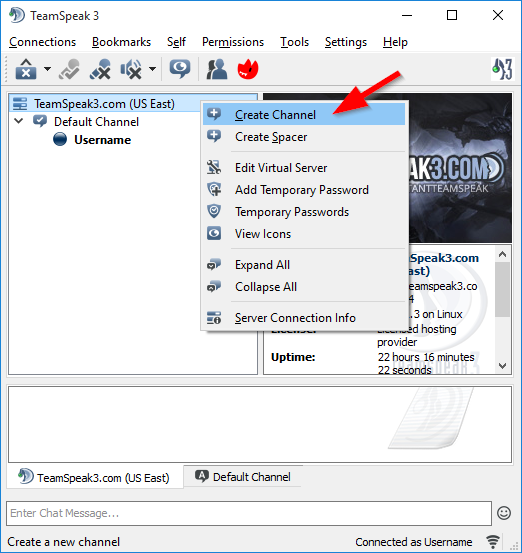
\includegraphics[width=0.78\textwidth,keepaspectratio]{figures/chapter3/ch3_fig02.png}
	\caption{Referencyjny układ TeamSpeak: serwer, kanały i czat kanału
		(źródło: \cite{TeamSpeak}).}
	\label{fig:ui_teamspeak}
\end{figure}

\begin{figure}[H]
	\centering
	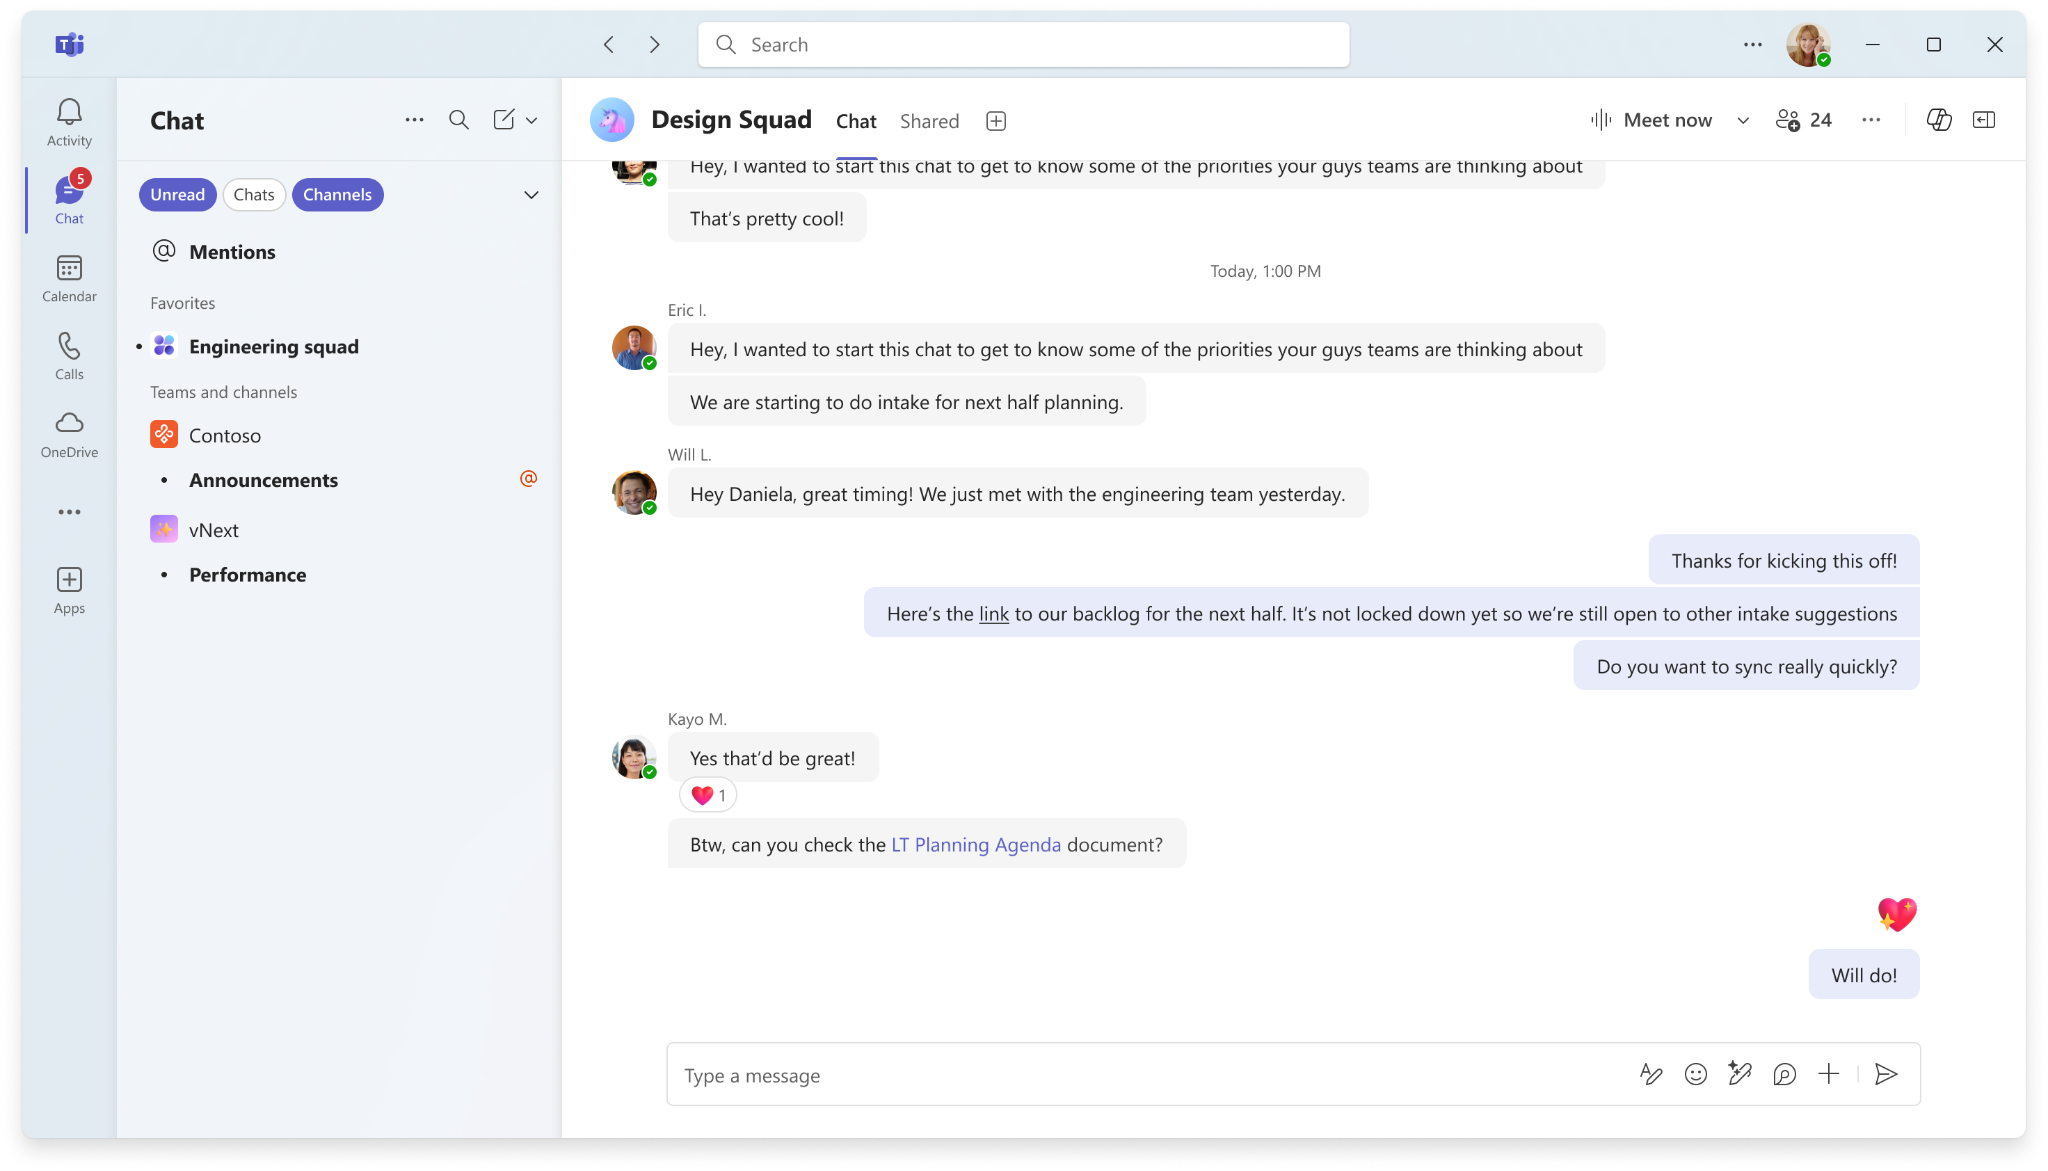
\includegraphics[width=0.95\textwidth,keepaspectratio]{figures/chapter3/ch3_fig03.png}
	\caption{Referencyjny układ Microsoft Teams: spotkanie, czat i udostępnianie
		treści (źródło: \cite{MSTeams}).}
	\label{fig:ui_teams}
\end{figure}

\begingroup
\scriptsize
\setlength{\LTpre}{6pt}
\setlength{\LTpost}{8pt}
\setlength{\tabcolsep}{3pt}
\renewcommand{\arraystretch}{1.18}
\begin{longtable}{|p{0.16\textwidth}|p{0.24\textwidth}|p{0.26\textwidth}|p{0.24\textwidth}|}
	\caption{Dobór inspiracji projektowych.}\label{tab:ui_inspiracje}\\
	\hline
	\textbf{Narzędzie} & \textbf{Dlaczego porównywane} & \textbf{Co wykorzystano} & \textbf{Co pozostaje poza zakresem} \\
	\hline
	\endfirsthead
	\hline
	\textbf{Narzędzie} & \textbf{Dlaczego porównywane} & \textbf{Co wykorzystano} & \textbf{Co pozostaje poza zakresem} \\
	\hline
	\endhead
	Discord & Popularny komunikator łączący głos, kanały, czat i pliki. &
	Układ panelu uczestników, czat, obsługa plików i drag-and-drop. &
	Rozbudowane społeczności, role, boty i serwery internetowe. \\
	\hline
	TeamSpeak & Lekka aplikacja głosowa z kanałami i niskim opóźnieniem. &
	Nacisk na głos, lista klientów i techniczna kontrola połączeń. &
	Zaawansowana administracja serwerem i system uprawnień. \\
	\hline
	Microsoft Teams & Platforma spotkań i pracy zespołowej. &
	Podział na uczestników, czat, pliki i zaproszenia. &
	Wideo, kalendarz, integracje chmurowe i organizacja firmowa. \\
	\hline
\end{longtable}
\endgroup

% ─────────────────────────────────────────────────────────────────────────────
\section{Schemat działania i przepływ pracy}
\label{sec:schemat_ui}
% ─────────────────────────────────────────────────────────────────────────────

Finalny interfejs obejmuje pełny przepływ użytkownika: ekran startowy,
formularz tworzenia pokoju, formularz dołączania, okno zaproszenia oraz
główny widok rozmowy. Taki podział jest czytelniejszy od wcześniejszego
widoku diagnostycznego, ponieważ użytkownik podejmuje najpierw decyzję
organizacyjną, a dopiero następnie przechodzi do rozmowy.

\begin{figure}[H]
	\centering
	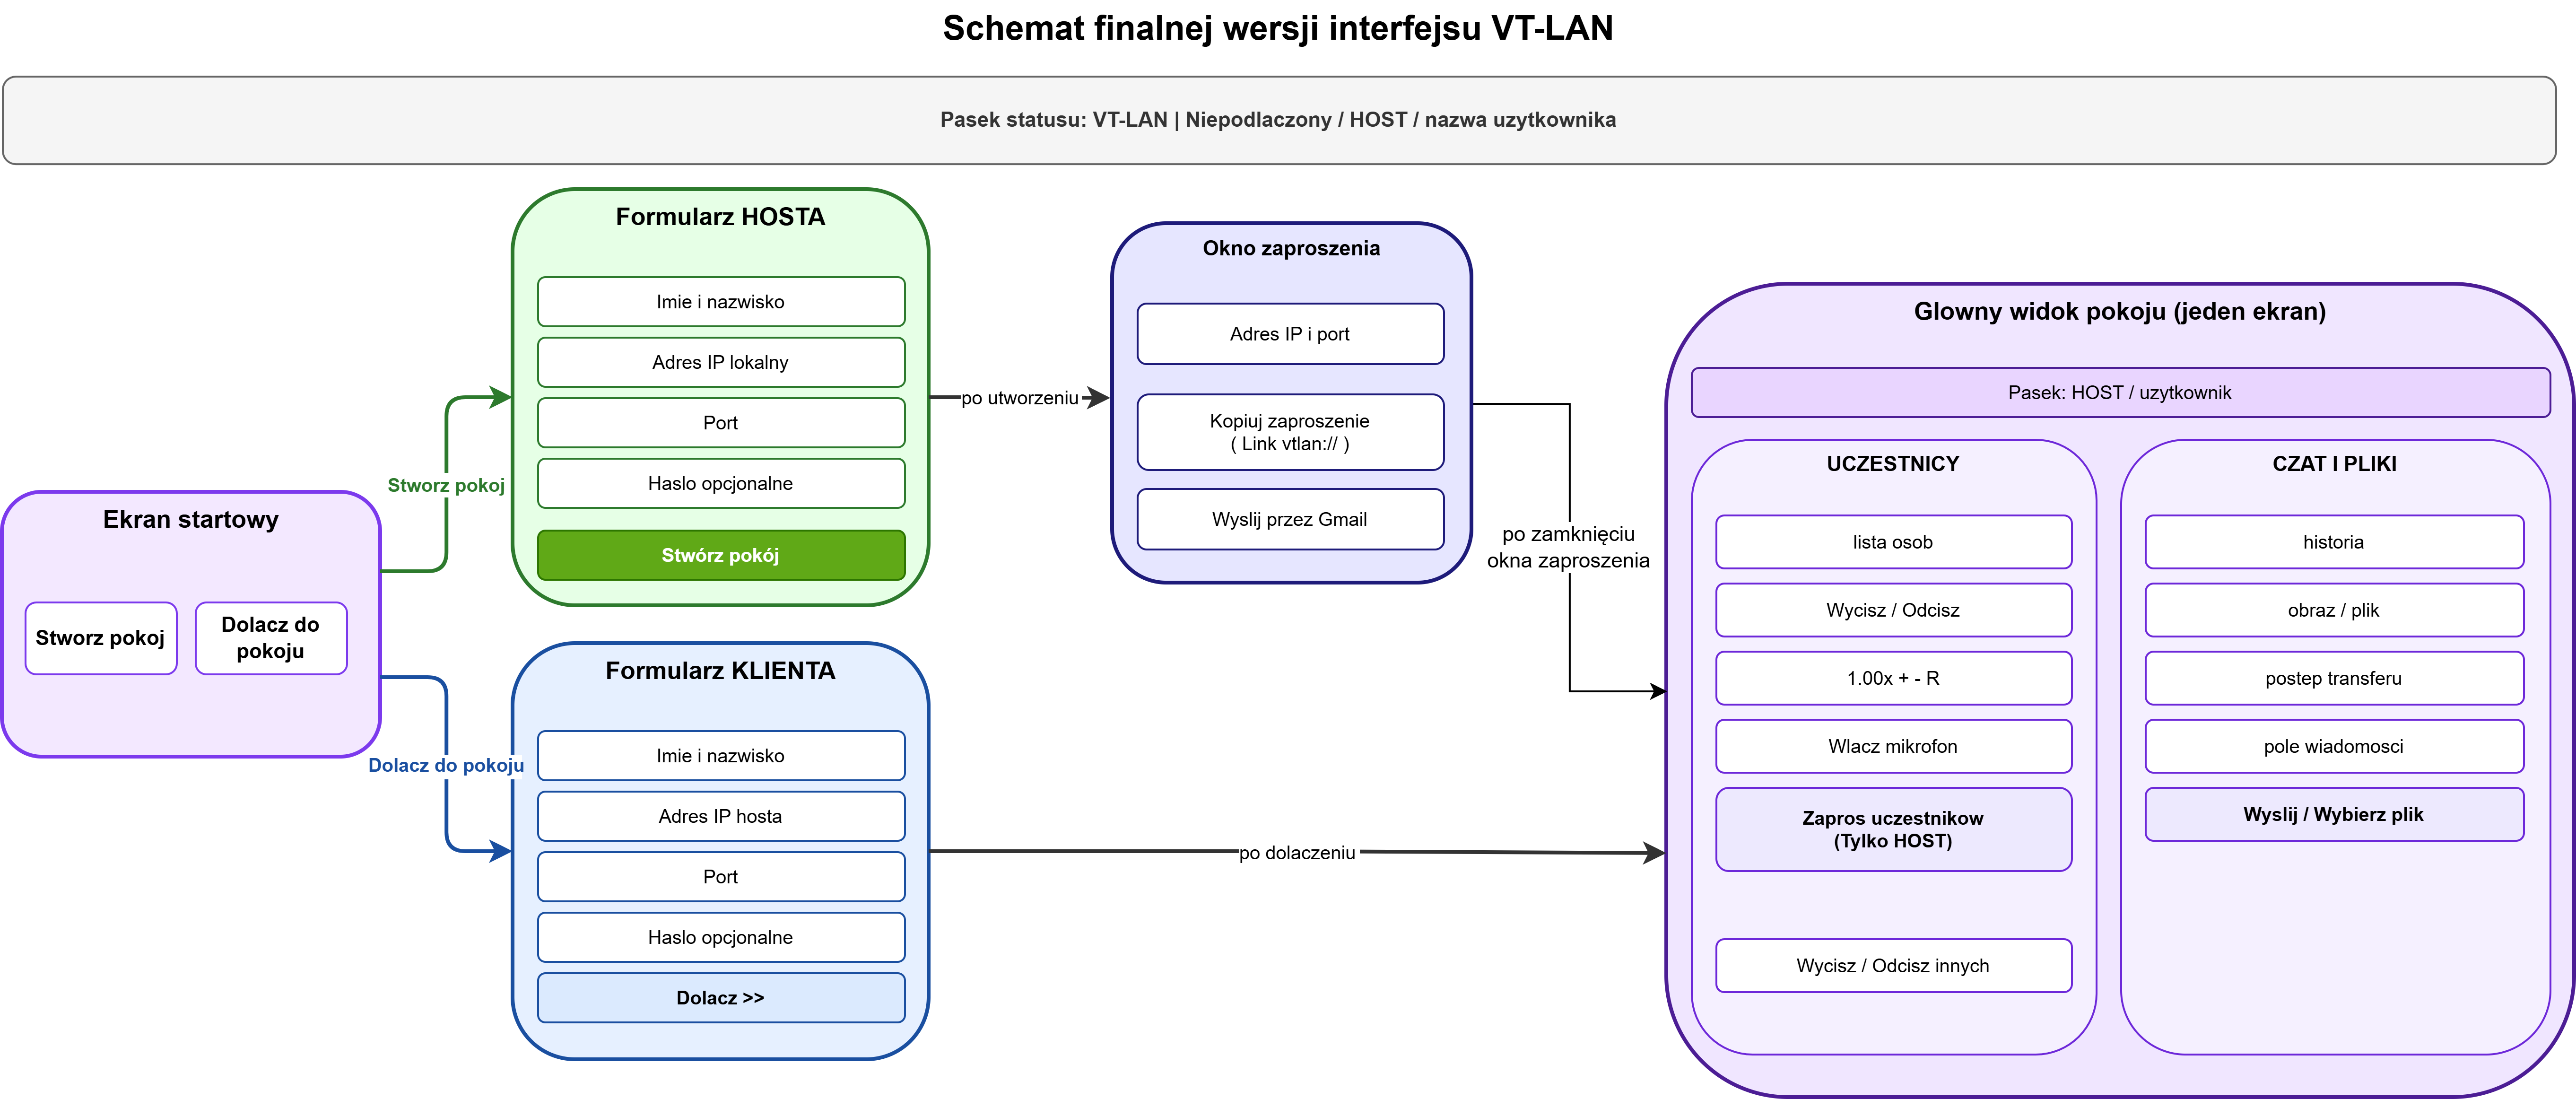
\includegraphics[width=1.0\textwidth,keepaspectratio]{figures/chapter3/ch3_fig04.png}
	\caption{Schemat blokowy finalnego interfejsu użytkownika. (praca własna)}
	\label{fig:ui_schemat_interfejsu}
\end{figure}

\begin{figure}[H]
	\centering
	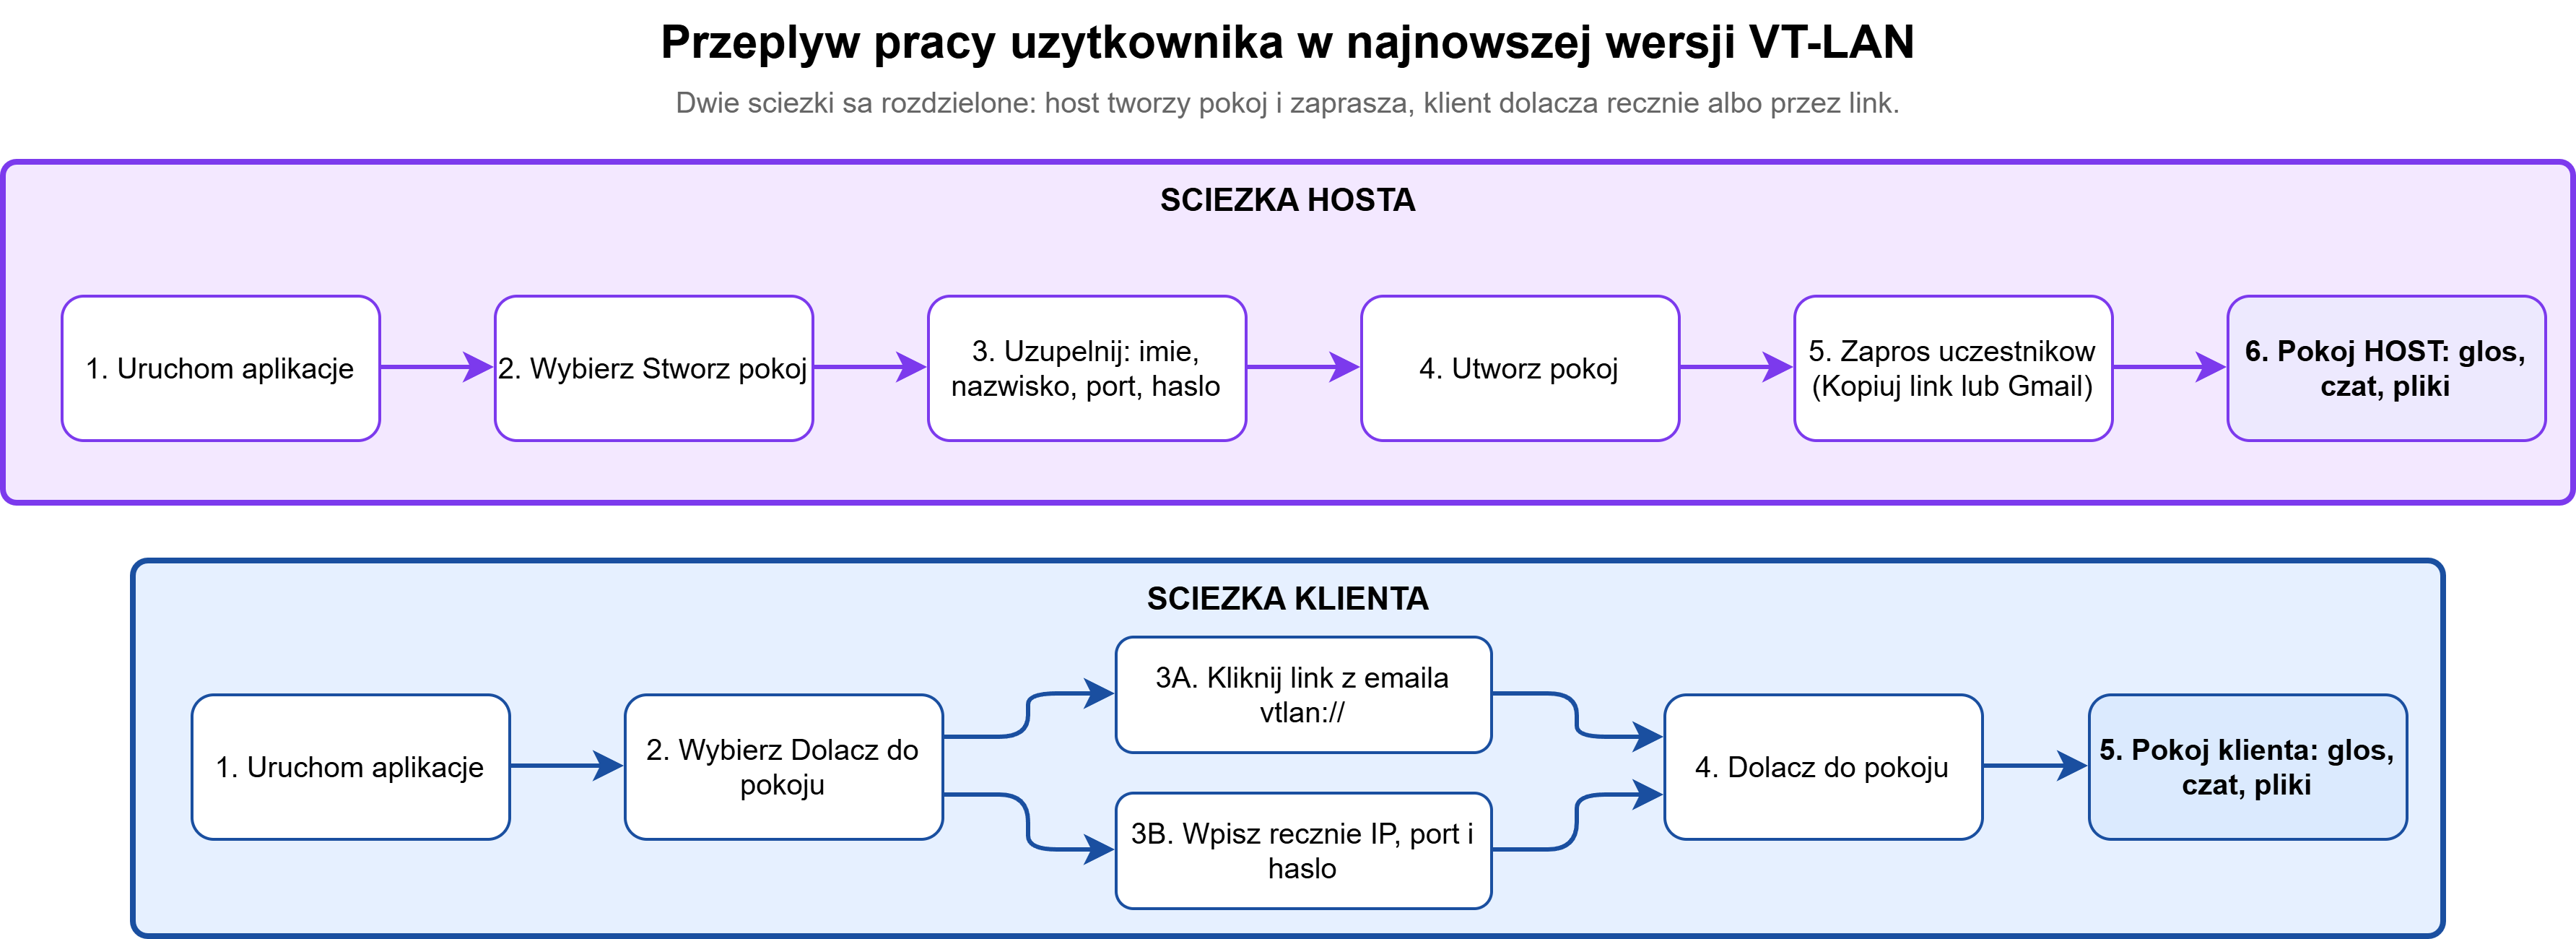
\includegraphics[width=0.95\textwidth,keepaspectratio]{figures/chapter3/ch3_fig05.png}
	\caption{Przepływ pracy użytkownika w finalnej wersji aplikacji. (praca własna)}
	\label{fig:ui_przeplyw_pracy}
\end{figure}

% ─────────────────────────────────────────────────────────────────────────────
\section{Ewolucja interfejsu w trakcie realizacji projektu}
\label{sec:rozwoj_ui}
% ─────────────────────────────────────────────────────────────────────────────

Interfejs aplikacji powstawał przyrostowo, równolegle z rozwojem warstwy
backendowej opisanej w rozdziale~\ref{chapt:Backend}. Najważniejsza zmiana
polegała na przejściu od narzędzia testowego do aplikacji użytkowej:
w pierwszych wersjach użytkownik od razu widział liczne elementy techniczne,
natomiast w finalnej wersji najpierw wybiera tryb pracy, a dopiero po
wejściu do pokoju widzi panel uczestników i czat.

\begin{figure}[H]
	\centering
	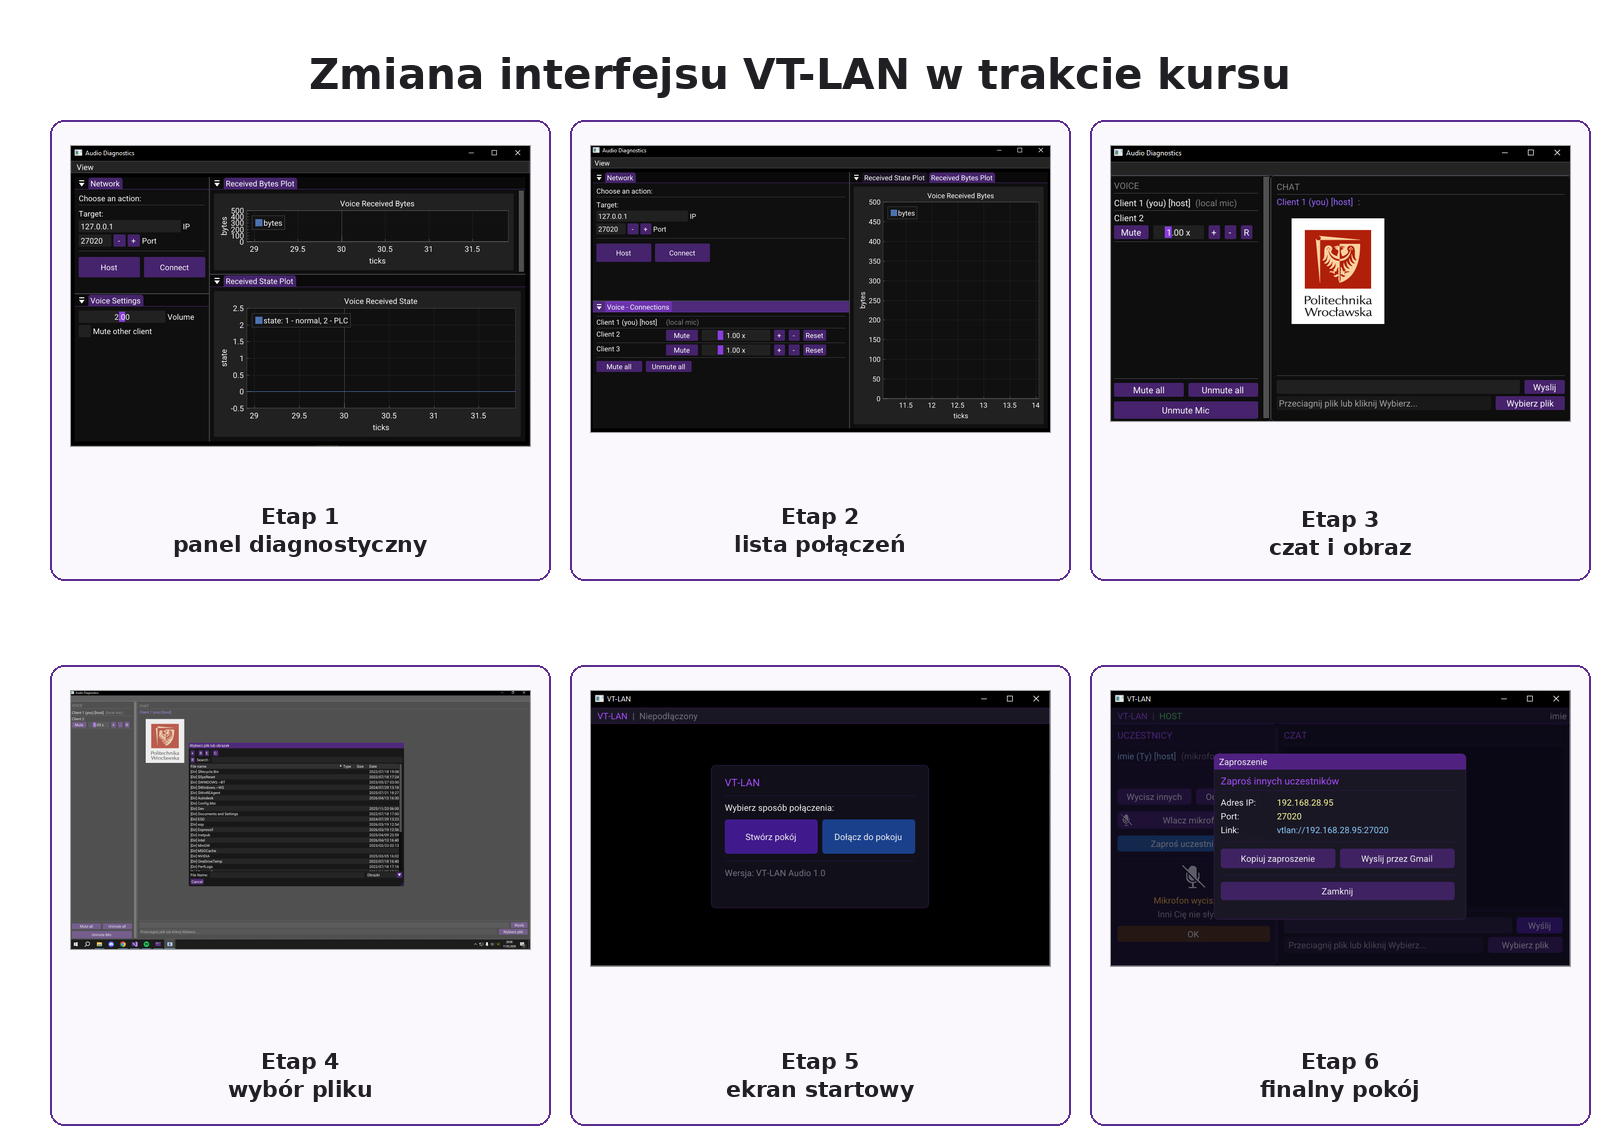
\includegraphics[width=1\textwidth,keepaspectratio]{figures/chapter3/ch3_fig06.png}
	\caption{Chronologiczna zmiana interfejsu VT-LAN w trakcie realizacji projektu. (praca własna)}
	\label{fig:ui_chronologia}
\end{figure}

\subsection{Etap 1 - panel diagnostyczny}
\label{subsec:etap1}

Pierwszy widok miał charakter czysto techniczny: pola adresu IP i portu,
przyciski trybu hosta i klienta, ustawienia audio oraz wykresy liczby
odebranych bajtów i stanu odbioru (rozumianego jako nagłówek pakietu głosowego \texttt{sequenceID} opisany w \ref{sec:voicecap}). Przeznaczony był dla twórców projektu
i umożliwiał weryfikację poprawności działania warstwy sieciowej
oraz modułu audio.

\begin{figure}[H]
	\centering
	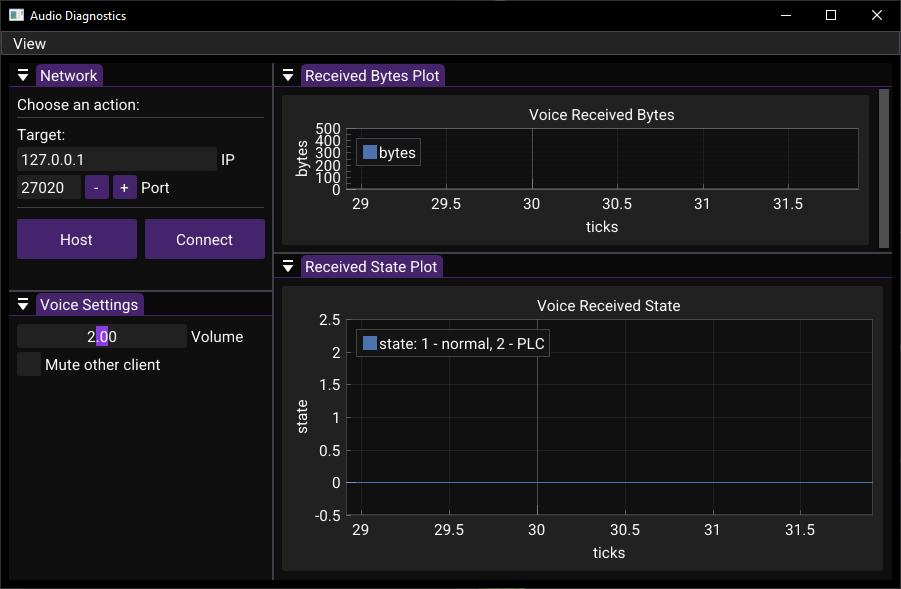
\includegraphics[width=0.95\textwidth,keepaspectratio]{figures/chapter3/ui_etap1_diagnostyczny.png}
	\caption{Etap 1 - panel diagnostyczny z ustawieniami sieci i wykresami transmisji. (praca własna)}
	\label{fig:ui_etap1}
\end{figure}

\subsection{Etap 2 - sterowanie połączeniami głosowymi}
\label{subsec:etap2}

W drugim etapie dodano panel \textit{Voice Connections} z listą aktywnych
klientów, oznaczeniem hosta i lokalnego mikrofonu oraz przyciskami
sterowania: \textit{Mute}, \textit{Reset}, \textit{Mute all}
i \textit{Unmute all}. Aplikacja umożliwiła prowadzenie rzeczywistej
rozmowy głosowej z kontrolą nad poszczególnymi uczestnikami.

\begin{figure}[H]
	\centering
	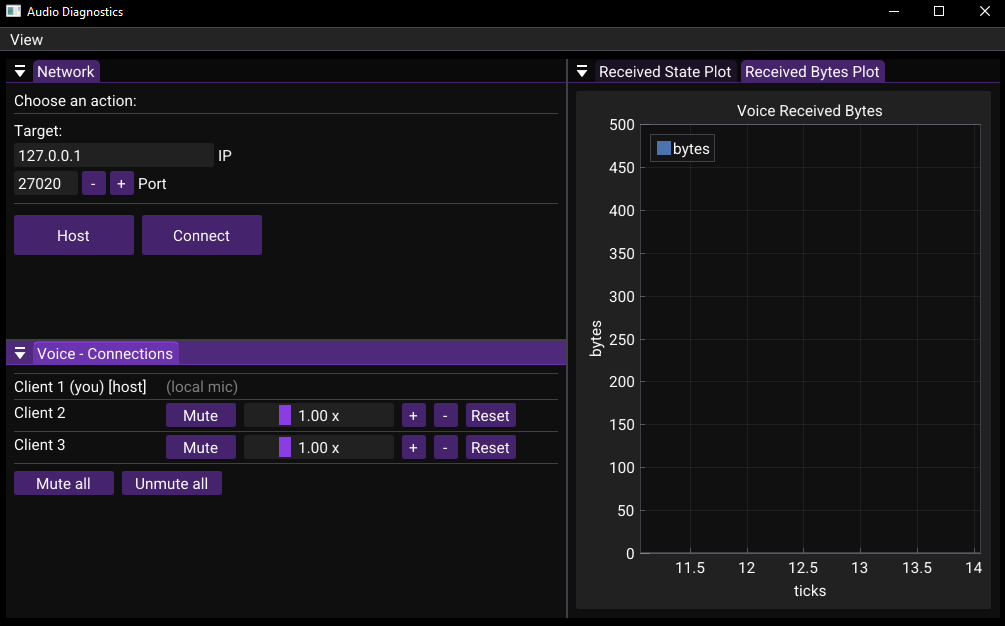
\includegraphics[width=0.95\textwidth,keepaspectratio]{figures/chapter3/ui_etap2_voice.png}
	\caption{Etap 2 - lista klientów i panel sterowania połączeniami głosowymi. (praca własna)}
	\label{fig:ui_etap2}
\end{figure}

\subsection{Etap 3 - czat tekstowy i podgląd obrazu}
\label{subsec:etap3}

Trzeci etap wprowadził panel czatu po prawej stronie ekranu. Obok historii
wiadomości dodano obsługę podglądu obrazów bezpośrednio w historii rozmowy,
bez potrzeby otwierania zewnętrznej przeglądarki. Dwupanelowy układ
ustalony na tym etapie zachowano w finalnej wersji aplikacji.

\begin{figure}[H]
	\centering
	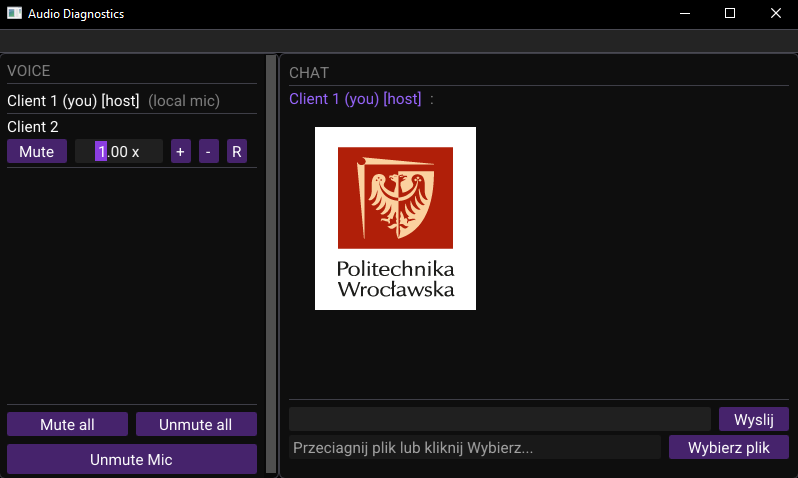
\includegraphics[width=0.95\textwidth,keepaspectratio]{figures/chapter3/ui_etap3_chat_obraz.png}
	\caption{Etap 3 - panel czatu z historią rozmowy i podglądem przesłanego obrazu. (praca własna)}
	\label{fig:ui_etap3}
\end{figure}

\subsection{Etap 4 - przesyłanie plików}
\label{subsec:etap4}

W czwartym etapie zaimplementowano dwie metody dodawania plików: przez
systemowe okno wyboru oraz przez przeciągnięcie pliku do obszaru czatu
(drag-and-drop). Techniczne szczegóły obsługi zdarzenia
\texttt{SDL\_EVENT\_DROP\_FILE} opisano w sekcji~\ref{sec:sdl}.

\begin{figure}[H]
	\centering
	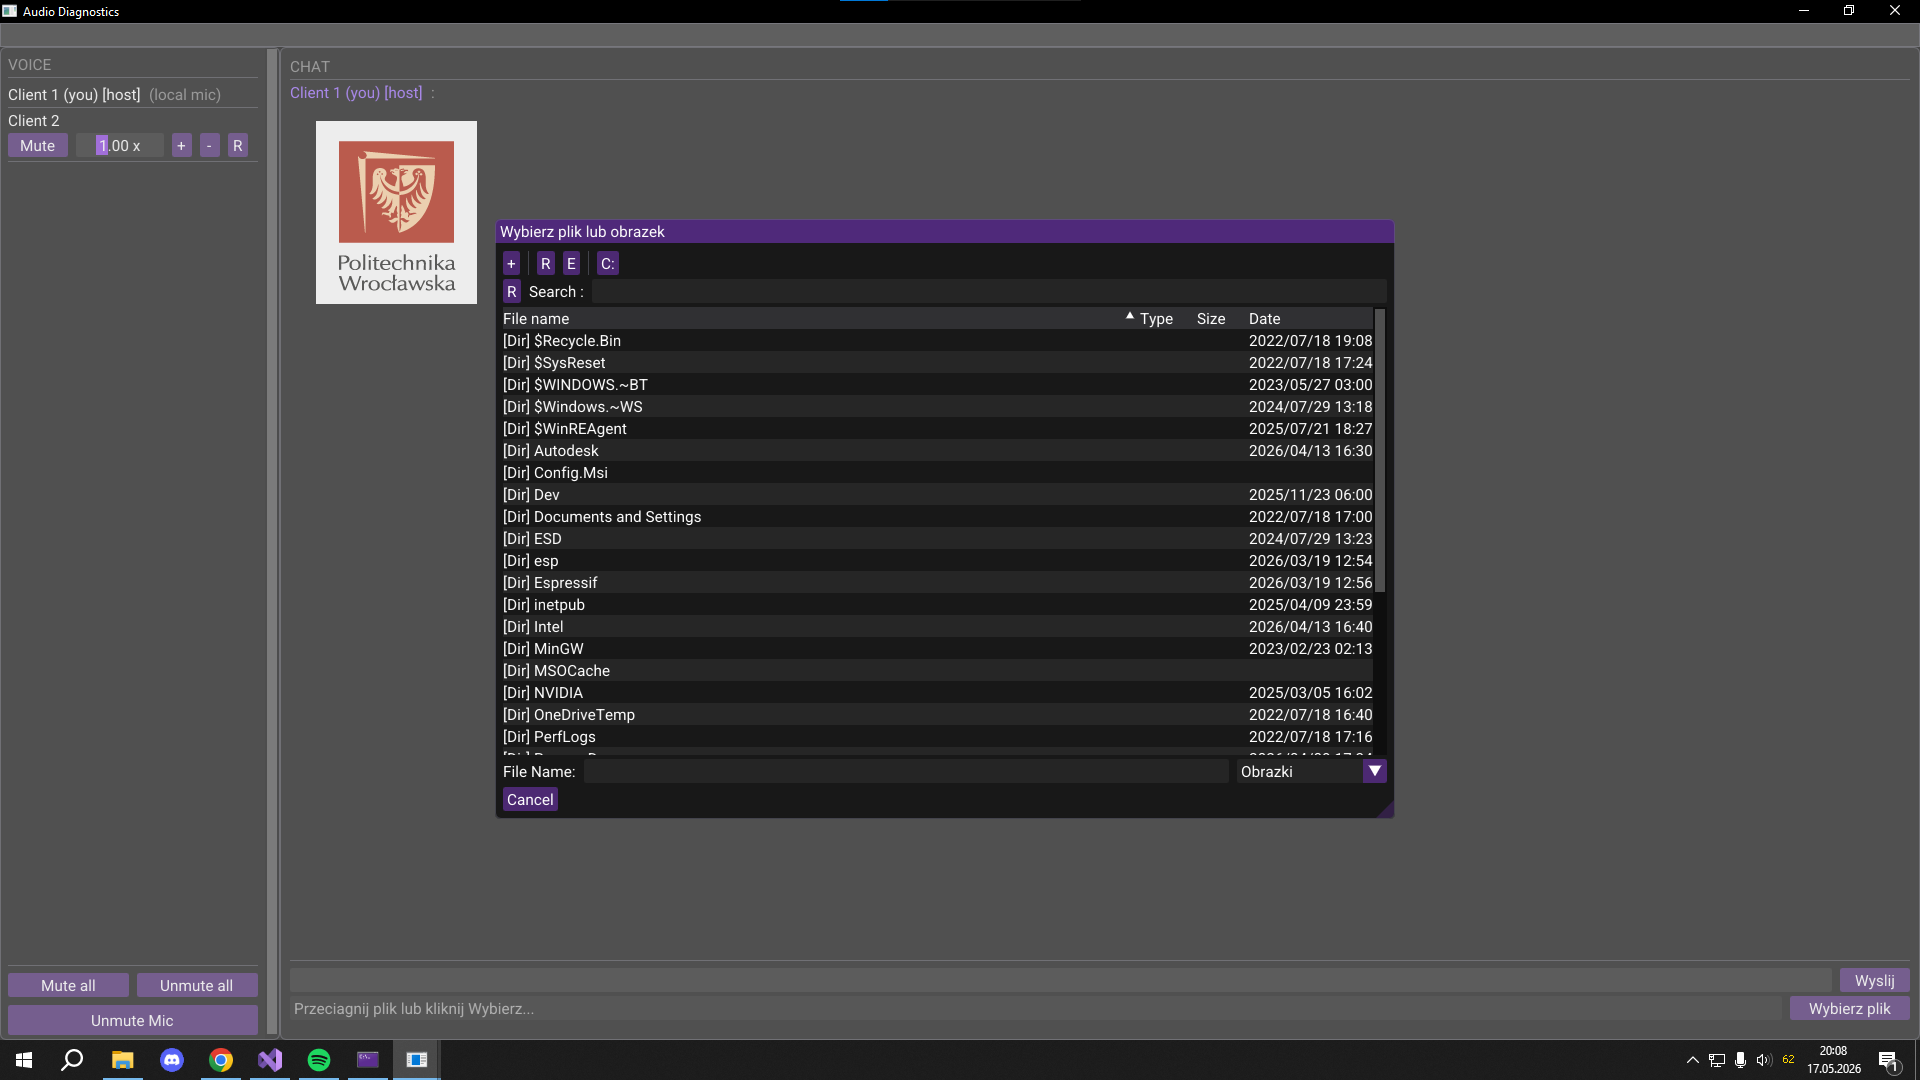
\includegraphics[width=0.95\textwidth,keepaspectratio]{figures/chapter3/ui_etap4_pliki.png}
	\caption{Etap 4 - okno wyboru pliku i obsługa załączników. (praca własna)}
	\label{fig:ui_etap4}
\end{figure}

% ─────────────────────────────────────────────────────────────────────────────
\section{Finalna wersja interfejsu}
\label{sec:finalna_wersja_ui}
% ─────────────────────────────────────────────────────────────────────────────

\subsection{Ekran startowy}
\label{subsec:ekran_startowy}

Ekran startowy zawiera nazwę aplikacji, status połączenia oraz dwa
przyciski wyboru trybu pracy. Uproszczona forma ekranu pozwala
użytkownikowi podjąć decyzję bez znajomości szczegółów sieciowych.

\begin{figure}[H]
	\centering
	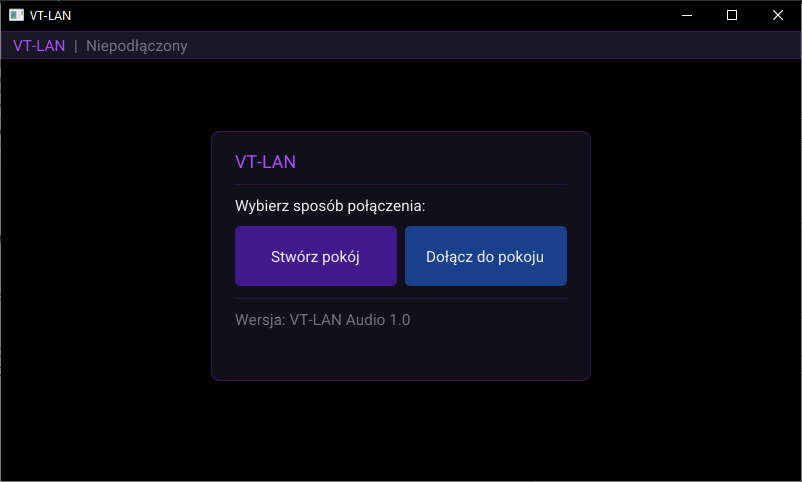
\includegraphics[width=0.88\textwidth,keepaspectratio]{figures/chapter3/ch3_fig07.png}
	\caption{Ekran startowy z wyborem sposobu dołączenia do sesji. (praca własna)}
	\label{fig:ui_ekran_startowy}
\end{figure}

\begingroup
\small
\setlength{\LTpre}{6pt}
\setlength{\LTpost}{8pt}
\setlength{\tabcolsep}{3pt}
\renewcommand{\arraystretch}{1.18}
\begin{longtable}{|p{0.22\textwidth}|p{0.34\textwidth}|p{0.34\textwidth}|}
	\caption{Elementy ekranu startowego.}\label{tab:ui_ekran_startowy}\\
	\hline
	\textbf{Element} & \textbf{Funkcja} & \textbf{Znaczenie} \\
	\hline
	\endfirsthead
	\hline
	\textbf{Element} & \textbf{Funkcja} & \textbf{Znaczenie} \\
	\hline
	\endhead
	VT-LAN | Niepodłączony & Nazwa programu i status połączenia. &
	Użytkownik od razu widzi, że nie jest jeszcze w pokoju. \\
	\hline
	Stwórz pokój & Uruchamia ścieżkę hosta. &
	Wyraźny wybór dla osoby rozpoczynającej sesję. \\
	\hline
	Dołącz do pokoju & Uruchamia ścieżkę klienta. &
	Wyraźny wybór dla osoby zaproszonej. \\
	\hline
	Wersja programu & Informuje o wersji aplikacji. &
	Przydatne przy testowaniu i dokumentowaniu projektu. \\
	\hline
\end{longtable}
\endgroup

\subsection{Tworzenie pokoju}
\label{subsec:tworzenie_pokoju}

Formularz tworzenia pokoju zbiera dane niezbędne do uruchomienia sesji:
imię i nazwisko hosta, lokalny adres IP, numer portu oraz opcjonalne
hasło pokoju maskowane gwiazdkami. Zaimplementowano walidację pól
wymaganych - przy braku danych program wyświetla komunikat informujący,
które pole wymaga uzupełnienia. Dane użytkownika są zapisywane
w pliku \texttt{user\_profile.txt} i automatycznie uzupełniane
przy kolejnym uruchomieniu.

\begin{figure}[H]
	\centering
	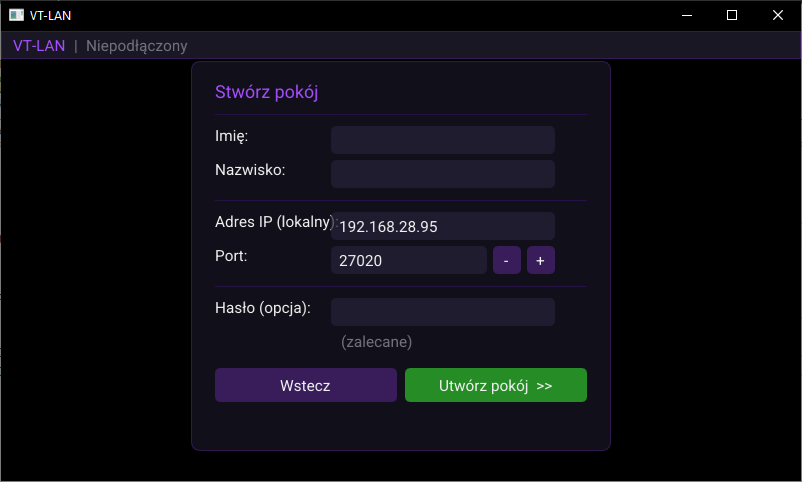
\includegraphics[width=0.88\textwidth,keepaspectratio]{figures/chapter3/ch3_fig08.png}
	\caption{Formularz tworzenia pokoju. (praca własna)}
	\label{fig:ui_tworzenie_pokoju}
\end{figure}

\subsection{Dołączanie do pokoju}
\label{subsec:dolaczanie}

Formularz dołączania przeznaczony jest dla uczestnika zaproszonego do
sesji. Pola adresu IP i portu mogą zostać uzupełnione ręcznie lub
automatycznie przez kliknięcie linku w formacie \texttt{vtlan://} -
obsługa inicjacji sesji opisana jest w sekcji~\ref{sec:tcp}.

\begin{figure}[H]
	\centering
	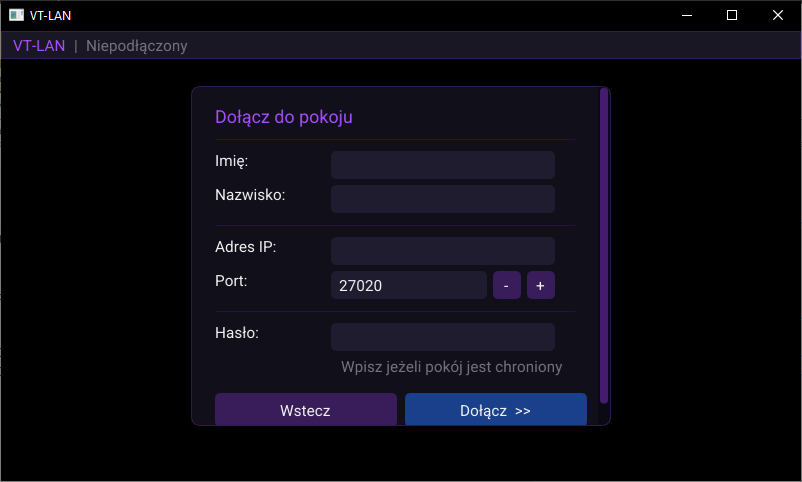
\includegraphics[width=0.88\textwidth,keepaspectratio]{figures/chapter3/ch3_fig10.png}
	\caption{Formularz dołączania do pokoju. (praca własna)}
	\label{fig:ui_dolaczanie}
\end{figure}

\begingroup
\small
\setlength{\LTpre}{6pt}
\setlength{\LTpost}{8pt}
\setlength{\tabcolsep}{3pt}
\renewcommand{\arraystretch}{1.18}
\begin{longtable}{|p{0.22\textwidth}|p{0.34\textwidth}|p{0.34\textwidth}|}
	\caption{Pola formularza dołączania do pokoju.}\label{tab:ui_formularz_dolaczania}\\
	\hline
	\textbf{Pole} & \textbf{Opis} & \textbf{Uwagi} \\
	\hline
	\endfirsthead
	\hline
	\textbf{Pole} & \textbf{Opis} & \textbf{Uwagi} \\
	\hline
	\endhead
	Imię i nazwisko & Identyfikuje użytkownika na liście uczestników. &
	Pole wymagane; dane mogą być zapamiętane lokalnie. \\
	\hline
	Adres IP & Adres hosta pokoju. &
	Uzupełniany ręcznie lub pobrany z linku \texttt{vtlan://}. \\
	\hline
	Port & Numer portu połączenia. &
	Domyślnie 27020; przyciski + i - ułatwiają zmianę. \\
	\hline
	Hasło & Opcjonalna ochrona dostępu do pokoju. &
	Wymagane gdy host ustawił hasło przy tworzeniu sesji. \\
	\hline
	Dołącz >> & Inicjuje próbę połączenia z pokojem. &
	Odróżniony kolorem od przycisku tworzenia pokoju. \\
	\hline
\end{longtable}
\endgroup

\subsection{Główny widok pokoju}
\label{subsec:glowny_widok}

Po wejściu do sesji użytkownik widzi główny ekran rozmowy. Lewy panel
\textit{Uczestnicy} zawiera listę osób, sterowanie głosem i przycisk
zaproszenia. Prawy panel \textit{Czat} zawiera historię wiadomości,
obrazy, informacje o plikach i pole wysyłania. Pasek statusu na górze
ekranu pokazuje tryb pracy (HOST lub CLIENT) oraz nazwę użytkownika.

\begin{figure}[H]
	\centering
	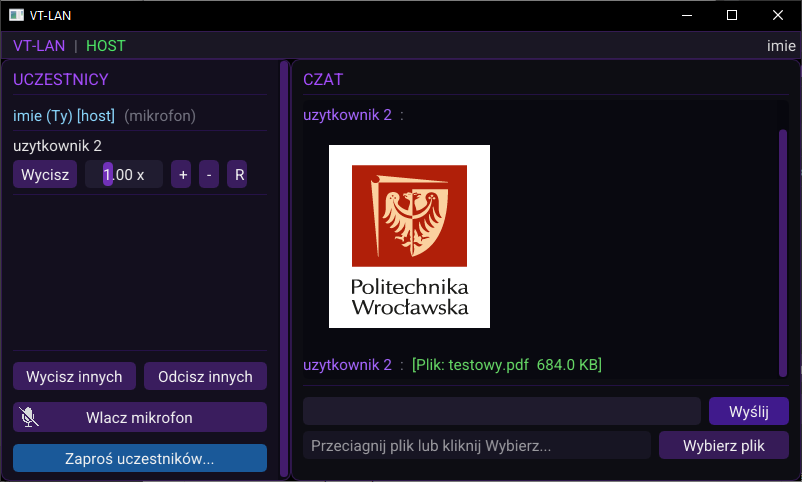
\includegraphics[width=0.88\textwidth,keepaspectratio]{figures/chapter3/ch3_fig11.png}
	\caption{Główny widok pokoju z panelem uczestników, czatem i plikami. (praca własna)}
	\label{fig:ui_glowny_pokoj}
\end{figure}

\begingroup
\small
\setlength{\LTpre}{6pt}
\setlength{\LTpost}{8pt}
\setlength{\tabcolsep}{3pt}
\renewcommand{\arraystretch}{1.18}
\begin{longtable}{|p{0.22\textwidth}|p{0.34\textwidth}|p{0.34\textwidth}|}
	\caption{Elementy głównego widoku pokoju.}\label{tab:ui_glowny_widok}\\
	\hline
	\textbf{Element} & \textbf{Funkcja} & \textbf{Znaczenie} \\
	\hline
	\endfirsthead
	\hline
	\textbf{Element} & \textbf{Funkcja} & \textbf{Znaczenie} \\
	\hline
	\endhead
	Pasek HOST/CLIENT & Wskazuje tryb pracy i nazwę użytkownika. &
	Pozwala odróżnić hosta od klienta na pierwszy rzut oka. \\
	\hline
	Lista uczestników & Wyświetla hosta, lokalny mikrofon i pozostałych klientów. &
	Kontrola składu aktywnej sesji. \\
	\hline
	Wycisz / Odcisz & Steruje dźwiękiem wybranego uczestnika lokalnie. &
	Kontrola dźwięku bez rozłączania połączenia. \\
	\hline
	1.00x, +, -, R & Reguluje i resetuje poziom głośności klienta. &
	Wyrównanie głośności rozmówców. \\
	\hline
	Wycisz / Odcisz innych & Grupowe sterowanie dźwiękiem uczestników. &
	Przydatne przy zakłóceniach i testach. \\
	\hline
	Włącz mikrofon & Przywraca lokalny mikrofon po wyciszeniu. &
	Szybki powrót do rozmowy. \\
	\hline
	Zaproś uczestników & Otwiera okno zaproszenia. &
	Ułatwia przekazanie danych pokoju nowym uczestnikom. \\
	\hline
\end{longtable}
\endgroup

% ─────────────────────────────────────────────────────────────────────────────
\section{Mechanizm zaproszeń}
\label{sec:zaproszenia_ui}
% ─────────────────────────────────────────────────────────────────────────────

Po kliknięciu przycisku \textit{Zaproś uczestników} host widzi okno
z adresem IP, numerem portu i linkiem w formacie \texttt{vtlan://adres:port}.
Dostępne są dwa sposoby przekazania zaproszenia: skopiowanie treści
do schowka systemowego lub otwarcie przygotowanej wiadomości w kliencie
Gmail. Wiadomość zawiera zarówno link \texttt{vtlan://}, jak i parametry
awaryjne (adres IP i port) na wypadek, gdy protokół nie jest obsługiwany
przez system operacyjny odbiorcy. Gmail służy wyłącznie do przekazania
zaproszenia - właściwa komunikacja odbywa się w całości w sieci lokalnej.

\begin{figure}[H]
	\centering
	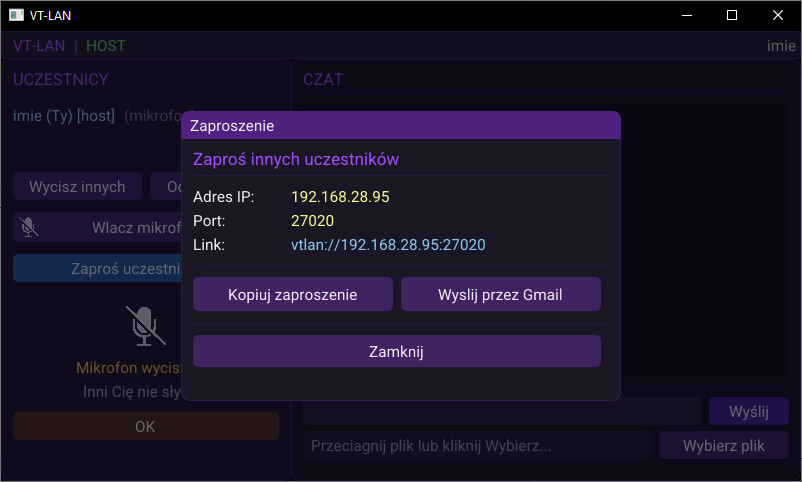
\includegraphics[width=0.88\textwidth,keepaspectratio]{figures/chapter3/ch3_fig12.png}
	\caption{Okno zaproszenia w panelu hosta. (praca własna)}
	\label{fig:ui_zaproszenie}
\end{figure}

\begin{figure}[H]
	\centering
	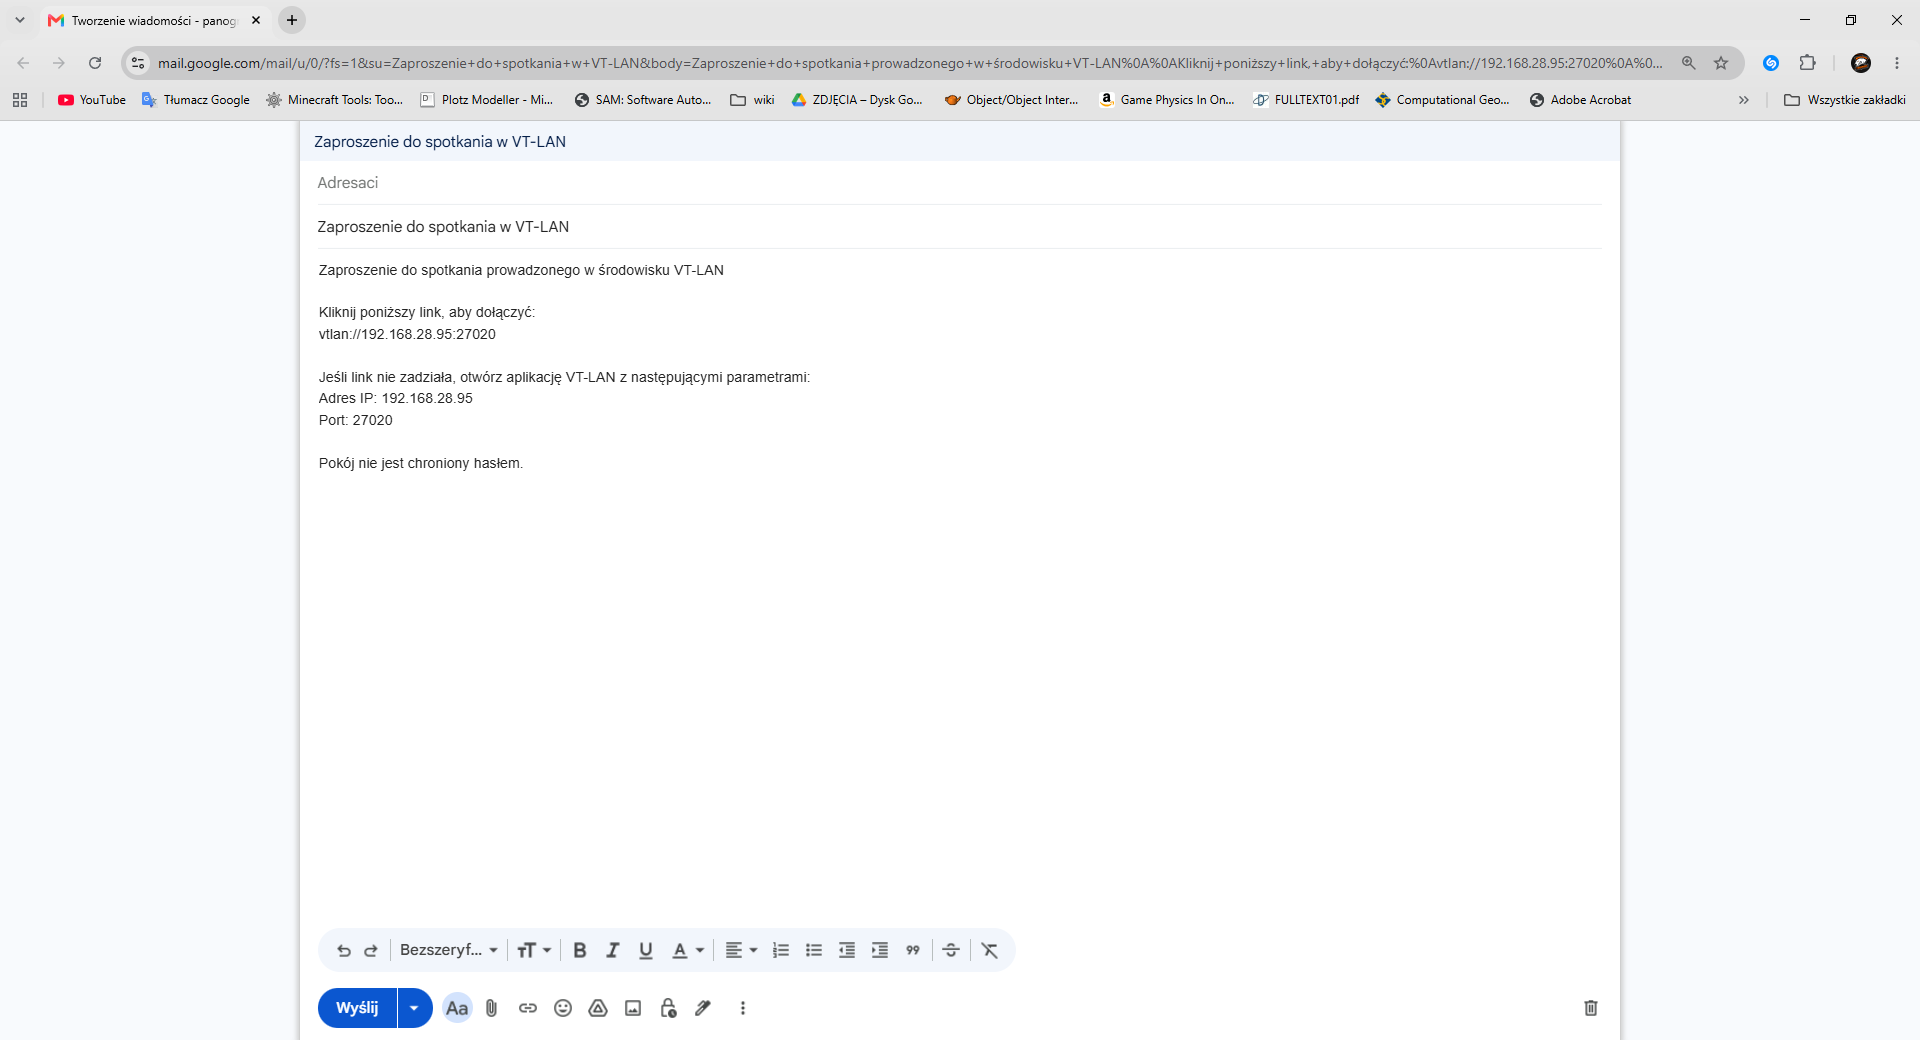
\includegraphics[width=0.88\textwidth,keepaspectratio]{figures/chapter3/ch3_fig13.png}
	\caption{Wiadomość Gmail wygenerowana przez funkcję zaproszenia. (praca własna)}
	\label{fig:ui_gmail}
\end{figure}

\begingroup
\small
\setlength{\LTpre}{6pt}
\setlength{\LTpost}{8pt}
\setlength{\tabcolsep}{3pt}
\renewcommand{\arraystretch}{1.18}
\begin{longtable}{|p{0.22\textwidth}|p{0.34\textwidth}|p{0.34\textwidth}|}
	\caption{Elementy okna zaproszenia.}\label{tab:ui_zaproszenie}\\
	\hline
	\textbf{Element} & \textbf{Opis} & \textbf{Znaczenie} \\
	\hline
	\endfirsthead
	\hline
	\textbf{Element} & \textbf{Opis} & \textbf{Znaczenie} \\
	\hline
	\endhead
	Adres IP i port & Dane połączenia hosta. &
	Umożliwiają ręczne dołączenie gdy link nie zadziała. \\
	\hline
	Link \texttt{vtlan://} & Protokół automatycznego dołączenia do pokoju. &
	Skraca proces dołączenia do kliknięcia linku. \\
	\hline
	Parametr \texttt{pwd=} & Opcjonalne hasło zakodowane w linku. &
	Przekazuje hasło pokoju wraz z zaproszeniem. \\
	\hline
	Kopiuj zaproszenie & Kopiuje treść zaproszenia do schowka. &
	Działa z dowolnym kanałem komunikacji. \\
	\hline
	Wyślij przez Gmail & Otwiera okno tworzenia wiadomości e-mail. &
	Wygodna metoda wysłania zaproszenia poza aplikacją. \\
	\hline
\end{longtable}
\endgroup

% ─────────────────────────────────────────────────────────────────────────────
\section{Funkcje czatu i przesyłania plików}
\label{sec:czat_pliki_ui}
% ─────────────────────────────────────────────────────────────────────────────

Panel czatu służy do wymiany wiadomości tekstowych, obrazów i plików.
Historia rozmowy wyświetla wiadomości, miniatury obrazów oraz nazwy
i rozmiary przesłanych plików. Podczas wysyłania dużego pliku widoczny
jest pasek postępu z nazwą pliku i liczbą przesłanych segmentów.
Odebrane pliki zapisywane są w katalogu \texttt{received\_files/}.
Szczegóły implementacji transferu (mechanizm RPC, segmentacja, rate-limiting)
opisano w sekcji~\ref{sec:tcp}.

\begin{figure}[H]
	\centering
	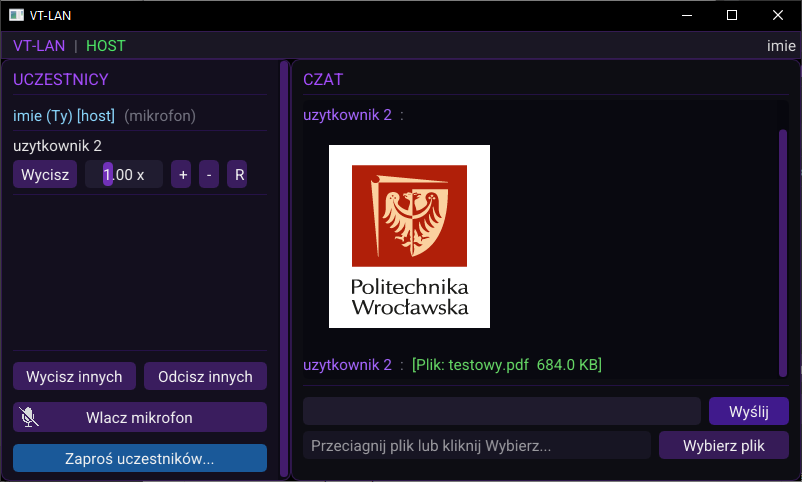
\includegraphics[width=0.88\textwidth,keepaspectratio]{figures/chapter3/ch3_fig14.png}
	\caption{Panel czatu z podglądem obrazu i informacją o przesłanym pliku PDF. (praca własna)}
	\label{fig:ui_czat_pdf}
\end{figure}

\begin{figure}[H]
	\centering
	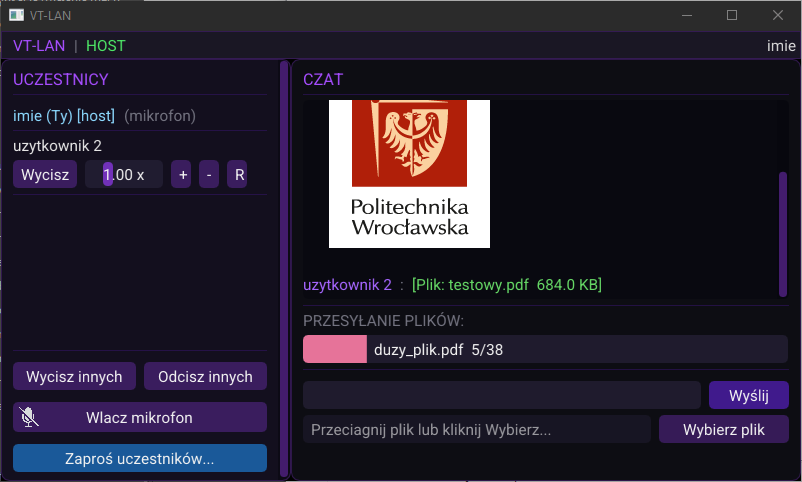
\includegraphics[width=0.88\textwidth,keepaspectratio]{figures/chapter3/ch3_fig15.png}
	\caption{Pasek postępu podczas przesyłania dużego pliku. (praca własna)}
	\label{fig:ui_postep}
\end{figure}

\begingroup
\small
\setlength{\LTpre}{6pt}
\setlength{\LTpost}{8pt}
\setlength{\tabcolsep}{3pt}
\renewcommand{\arraystretch}{1.18}
\begin{longtable}{|p{0.22\textwidth}|p{0.34\textwidth}|p{0.34\textwidth}|}
	\caption{Funkcje panelu czatu i przesyłania plików.}\label{tab:ui_czat_pliki}\\
	\hline
	\textbf{Funkcja} & \textbf{Opis działania} & \textbf{Efekt praktyczny} \\
	\hline
	\endfirsthead
	\hline
	\textbf{Funkcja} & \textbf{Opis działania} & \textbf{Efekt praktyczny} \\
	\hline
	\endhead
	Wiadomości tekstowe & Wpisywane w dolnym polu i wysyłane przyciskiem
	\textit{Wyślij}. & Szybka wymiana informacji podczas rozmowy. \\
	\hline
	Wybierz plik & Otwiera systemowe okno wyboru pliku. &
	Klasyczna metoda dodawania dokumentu z dysku. \\
	\hline
	Drag-and-drop & Plik przeciągany bezpośrednio do obszaru czatu. &
	Skraca czas dodawania pliku widocznego na pulpicie. \\
	\hline
	Podgląd obrazu & Miniatura grafiki widoczna w historii rozmowy. &
	Odbiorca ocenia zawartość bez otwierania zewnętrznej przeglądarki. \\
	\hline
	Informacja o pliku & Nazwa i rozmiar pliku wyświetlane w czacie. &
	Ułatwia weryfikację otrzymanego załącznika. \\
	\hline
	Pasek postępu & Nazwa pliku i liczba przesłanych segmentów. &
	Informuje o przebiegu transferu dużych plików. \\
	\hline
	Folder \texttt{received\_files} & Odebrane pliki zapisywane lokalnie. &
	Pliki dostępne po zakończeniu sesji. \\
	\hline
\end{longtable}
\endgroup

% ─────────────────────────────────────────────────────────────────────────────
\section{Porównanie funkcjonalne z innymi komunikatorami}
\label{sec:porownanie_ui}
% ─────────────────────────────────────────────────────────────────────────────

Szczegółowa charakterystyka rozwiązań rynkowych przedstawiona jest
w sekcji~\ref{sec:przeglad_rynku}. Poniższa tabela zestawia funkcje
istotne z perspektywy interfejsu i scenariusza użycia w sieci lokalnej.

\begingroup
\scriptsize
\setlength{\LTpre}{6pt}
\setlength{\LTpost}{8pt}
\setlength{\tabcolsep}{3pt}
\renewcommand{\arraystretch}{1.18}
\begin{longtable}{|p{0.19\textwidth}|p{0.12\textwidth}|p{0.17\textwidth}|p{0.19\textwidth}|p{0.19\textwidth}|}
	\caption{Porównanie funkcjonalne VT-LAN z wybranymi komunikatorami.}
	\label{tab:ui_porownanie}\\
	\hline
	\textbf{Funkcja} & \textbf{VT-LAN} & \textbf{Discord} &
	\textbf{TeamSpeak} & \textbf{MS Teams} \\
	\hline
	\endfirsthead
	\hline
	\textbf{Funkcja} & \textbf{VT-LAN} & \textbf{Discord} &
	\textbf{TeamSpeak} & \textbf{MS Teams} \\
	\hline
	\endhead
	Rozmowa głosowa          & Tak & Tak & Tak & Tak \\
	\hline
	Czat tekstowy            & Tak & Tak & Ograniczony & Tak \\
	\hline
	Przesyłanie plików       & Tak & Tak & Tak & Tak \\
	\hline
	Drag-and-drop            & Tak & Tak & Ograniczone & Tak \\
	\hline
	Podgląd obrazu w czacie  & Tak & Tak & Ograniczone & Tak \\
	\hline
	Zaproszenie linkiem      & Tak (\texttt{vtlan://}) & Tak & Tak & Tak \\
	\hline
	Działanie wyłącznie w LAN & Tak & Nie & Możliwe & Nie \\
	\hline
	Brak konta chmurowego    & Tak & Nie & Zależnie od konfiguracji & Nie \\
	\hline
	Hasło pokoju             & Tak & Zależnie od serwera & Tak & Zależnie od ustawień \\
	\hline
	Rozmowy wideo            & Nie & Tak & Nie & Tak \\
	\hline
	Transmisja ekranu        & Nie & Tak & Nie & Tak \\
	\hline
	Narzut zasobów           & Niski & Wysoki & Niski & Wysoki \\
	\hline
\end{longtable}
\endgroup

Przewaga VT-LAN wynika z dopasowania do lokalnego scenariusza LAN:
brak wymogu kont i zewnętrznej infrastruktury, niskie zużycie zasobów
(potwierdzone w rozdziale~\ref{ch:profilowanie_debugging}) oraz pełna
kontrola nad danymi. Brak wideo i transmisji ekranu stanowi świadomy
wybór projektowy, a nie ograniczenie - elementy te opisano jako
kierunki dalszej rozbudowy w poniższej sekcji.

% ─────────────────────────────────────────────────────────────────────────────
\section{Kierunki dalszego rozwoju}
\label{sec:dalsza_rozbudowa_ui}
% ─────────────────────────────────────────────────────────────────────────────

\begingroup
\small
\setlength{\LTpre}{6pt}
\setlength{\LTpost}{8pt}
\setlength{\tabcolsep}{3pt}
\renewcommand{\arraystretch}{1.2}
\begin{longtable}{|p{0.26\textwidth}|p{0.32\textwidth}|p{0.30\textwidth}|}
	\caption{Elementy poza bieżącym zakresem i możliwe kierunki rozwoju.}
	\label{tab:ui_dalszy_rozwoj}\\
	\hline
	\textbf{Element} & \textbf{Powód pominięcia} & \textbf{Kierunek rozwoju} \\
	\hline
	\endfirsthead
	\hline
	\textbf{Element} & \textbf{Powód pominięcia} & \textbf{Kierunek rozwoju} \\
	\hline
	\endhead
	Wideokonferencje & Zwiększa wymagania przepustowości i złożoność kodowania. &
	Moduł kamery z kodekiem wideo po stronie backendu. \\
	\hline
	Transmisja ekranu & Wymaga przechwytywania pulpitu i obsługi większego strumienia. &
	Prosta transmisja ekranu hosta do uczestników w LAN. \\
	\hline
	Lokalne konta użytkowników & Szybsze uruchomienie bez rejestracji. &
	Profile lokalne z rolami hosta i uczestnika. \\
	\hline
	Historia sesji & Nacisk na bieżącą komunikację w LAN. &
	Lokalny zapis historii lub baza SQLite. \\
	\hline
	Panel ustawień audio & Wybór urządzenia odbywa się domyślnie. &
	Wybór urządzenia wejściowego z testem poziomu sygnału. \\
	\hline
	Indykator szyfrowania w UI & Szyfrowanie działa transparentnie przez GNS. &
	Ikona bezpieczeństwa z informacją o trybie połączenia. \\
	\hline
\end{longtable}
\endgroup

% ─────────────────────────────────────────────────────────────────────────────
\section{Podsumowanie}
\label{sec:podsumowanie_ui}
% ─────────────────────────────────────────────────────────────────────────────

Finalna wersja VT-LAN stanowi spójny komunikator LAN z kompletnym
przepływem użytkownika: od ekranu startowego i formularzy sesji, przez
główny pokój rozmowy z kontrolą głosu, czatem i plikami, po mechanizm
zaproszenia przez link \texttt{vtlan://} lub wiadomość e-mail.
Każdy etap rozwoju interfejsu był ściśle powiązany z rozbudową warstwy
backendowej opisanej w rozdziale~\ref{chapt:Backend}.

Projekt realizuje podstawowy zestaw funkcji komunikatora LAN przy niskim
narzucie zasobów i prostym modelu obsługi - bez wymogu kont zewnętrznych
ani dostępu do Internetu w trakcie sesji. Brak wideo, transmisji ekranu
i rozbudowanych uprawnień to świadoma decyzja projektowa, a wymienione
elementy stanowią logiczny kierunek dalszej rozbudowy aplikacji.

\flushbottom 